\section{Συμπίεση Δεδομένων} \label{sec:data_compression}
\noindent
Σε αυτή την ενότητα, αναλύονται τα βήματα που ακολουθήθηκαν για την μείωση των δεδομένων των αμφιωτικών παραμέτρων, καθώς και τα κίνητρα πίσω από αυτή. Έγινε προσπάθεια για την επίτευξη της μέγιστης ευελιξίας, λόγω των δεδομένων, ως προς τις δομές των ΝΝ που μπορούσαν να χρησιμοποιηθούν, αφού μεγάλα παραδείγματα εισόδου, εισάγουν περιορισμούς ως προς το πλήθος των κρυφών επιπέδων που μπορούν να χρησιμοποιηθούν, αλλά και το πλήθος των νευρώνων σε κάθε ένα από αυτά. Η συμπίεση συμβαίνει σε δύο στάδια. Στο πρώτο, τα δεδομένα συμπιέζονται με βάση με βάση ψυχοακουστικά μοντέλα ως προς την αντίληψη του ήχου, που υποδεικνύουν τις σημαντικές μπάντες κάθε παραμέτρου, ενώ στο δεύτερο εφαρμόζεται ο αλγόριθμος συμπίεσης που σχεδιάστηκε, για την εξαγωγή των 'προφίλ' των παραμέτρων. Συνοπτικά η συμπίεση περιγράφεται στο Σχήμα \ref{fig:Compression_block_diagram}, όπου με $P$ σημειώνεται η παράμετρος ενδιαφέροντος, $N_{dim}$ οι αρχικές διαστάσεις της, και με $N'_{dim}$ οι μειωμένες διαστάσεις. Τα στοιχεία του διαγράμματος αναλύονται περαιτέρω στις επόμενες υποενότητες.

\begin{figure}[h]
  \centering
  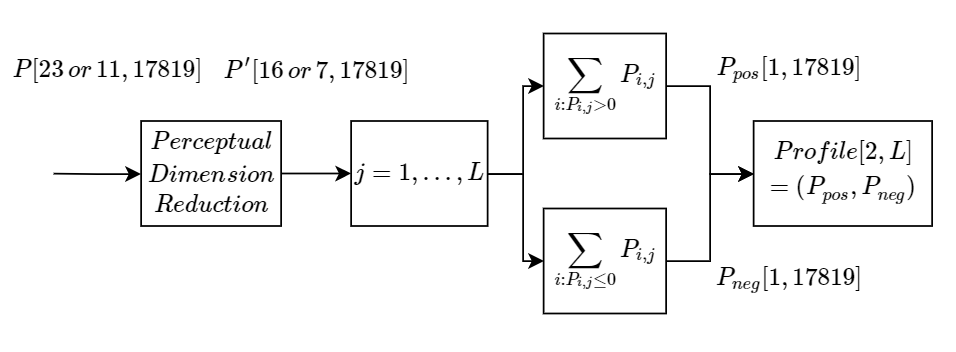
\includegraphics[width=\textwidth]{images/Compression_block_diagram.png}
  \caption{Προτεινόμενη μέθοδος συμπίεσης για τις αμφιωτικές παραμέτρους.}
  \label{fig:Compression_block_diagram}
\end{figure}

\subsection{Κίνητρο}

Για να γίνει σαφές το σκεπτικό πίσω από την επιλογή για τη συμπίεση των δεδομένων, είναι απαραίτητο να γίνει σαφές το μέγεθος των δεδομένων που το ακουστικό μοντέλο δίνει ως έξοδο. Όπως έχει αναφερθεί, το ILD έχει σε αυτό το σημείο 23 διαστάσεις και το ITD 11, κάθε μία από τις οποίες αντιστοιχεί σε μια μπάντα συχνοτήτων. Κάθε διάσταση έχει τον ίδιο αριθμό δειγμάτων με όλες τις υπόλοιπες, οπότε μπορούμε να πούμε ότι έχουμε συνολικά $23 + 11 = 34$ διαστάσεις δεδομένων. Το ακουστικό μοντέλο εκτελεί τις πράξεις της συνέλιξης, χωρίς να αυξάνει το πλήθος των δειγμάτων, οπότε κάθε διάσταση, όπως έχει αναφερθεί στην ενότητα \ref{sec:bin_sig_creation}, έχει $17819$, σημεία. Συνεπώς, προκύπτουν $34 * 17819 = 605846$ δείγματα. Γίνεται αμέσως αντιληπτό, πως το πλήθος των δειγμάτων, καθιστά το διάνυσμα απαγορευτικό για χρήση στην εκπαίδευση ενός νευρωνικού δικτύου, τόσο από άποψη του χρόνου που θα απαιτούνταν για την εκπαίδευση ενός τέτοιου μοντέλου, όσο και από την άποψη των περιορισμένων υπολογιστικών πόρων που είναι διαθέσιμοι.

\subsection{Αντιληπτική Συμπίεση}

Όπως έχει αναφερθεί στην ενότητα \ref{sec:binaural_cues}, αναλόγως με τη συχνότητα, η κάθε παράμετρος αποκτά διαφορετική βαρύτητα στον εντοπισμό ακουστικών πηγών. Με το ILD, να παίζει μεγαλύτερο ρόλο στις συχνότητες που είναι μεγαλύτερες από $1500 Hz$, ενώ το ITD το αντίθετο. Με βάση τις εξόδους του μοντέλου, και τη γνώση ότι κάθε μία από τις διαστάσεις των παραμέτρων αντιστοιχεί σε πλάτος 1 ERB, είναι αρκετά εύκολο να γίνει η αντιστοίχηση διαστάσεων-συχνοτικών μπαντών. Σε αυτή την εργασία, το crossover frequency, αντί για $1500 Hz$ τέθηκε κοντά στα $2000 Hz$, ώστε να υπάρχει μεγαλύτερη ισορροπία στο πλήθος των σημείων του ITD και του ILD. Σημειώνεται και εδώ πως χρησιμοποιείται η envelope δομή του μοντέλου.
Πιο συγκεκριμένα, από το ILD διατηρούνται οι διαστάσεις $8-23$, ενώ από το ITD οι $1-7$, όπως φαίνεται στην Εξίσωση \ref{eq:compression_1}. Τα αποτελέσματα της αντιληπτικής συμπίεσης παρουσιάζονται στα Σχήματα \ref{fig:ILD_Perceptual_Comp} και \ref{fig:ITD_Perceptual_Comp}.

\begin{CEquation}
\begin{split}
    ILD_{new} = ILD[8:23,:]\\
    ITD_{new} = ITD[1:7,:]
    \label{eq:compression_1}
\end{split}
\end{CEquation}

\begin{figure}[h]
  \centering
  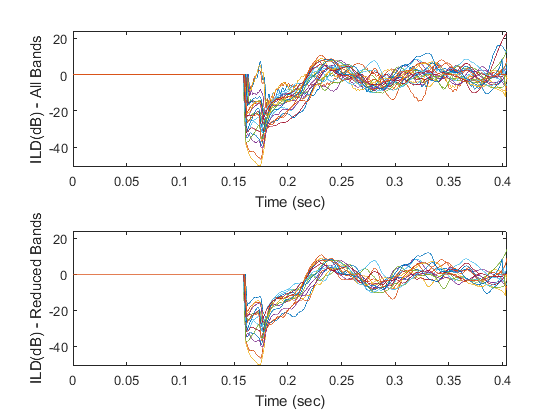
\includegraphics[width=\textwidth]{images/ILD_Perceptual_Comp.png}
  \caption{Σύγκριση πριν και μετά τη συμπίεση, της παραμέτρου ILD.}
  \label{fig:ILD_Perceptual_Comp}
\end{figure}

\begin{figure}[h]
  \centering
  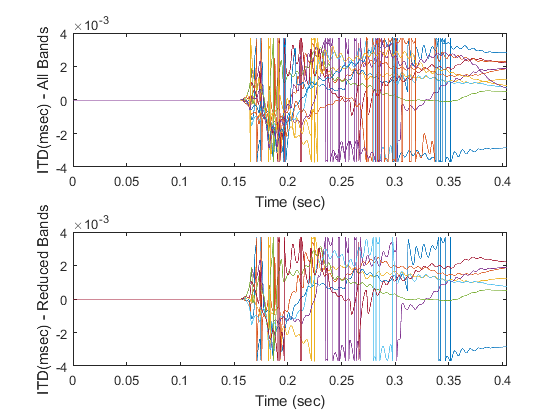
\includegraphics[width=\textwidth]{images/ITD_Perceptual_Comp.png}
  \caption{Σύγκριση πριν και μετά τη συμπίεση, της παραμέτρου ITD.}
  \label{fig:ITD_Perceptual_Comp}
\end{figure}

\sectionbreak
\subsection{Αλγοριθμική Συμπίεση}
Από τις παραμέτρους που προκύπτουν από την αντιληπτική συμπίεση, ο στόχος είναι ο υπολογισμός δύο χαρακτηριστικών καμπυλών, 'προφίλ', με σημαντικά μειωμένο μέγεθος δεδομένων, μία για τις θετικές και μία για τις αρνητικές τιμές κάθε παραμέτρου. Ο αλγόριθμος προσπελαύνει τις παραμέτρους ως προς το $L$, δηλαδή τη 'μεγάλη' διάσταση, και υπολογίζει δύο διαφορετικά αθροίσματα, ένα για τις θετικές τιμές κάθε διάστασης και ένα για τις αρνητικές, για το δείγμα $i$, και διαιρεί κάθε ένα από τα αθροίσματα με το πλήθος των στοιχείων που ανατέθηκαν σε αυτό, όπως φαίνεται στις Εξισώσεις \ref{eq:positive_profile} και \ref{eq:negative_profile}. Στη συνέχεια, τα δύο διανύσματα, συνδυάζονται στο τελικό προφίλ της παραμέτρου $Profile[2,L]$, όπως φαίνεται στην Εξίσωση \ref{eq:final_profile}. Τυπικά αποτελέσματα του αλγορίθμου φαίνονται στο Σχήμα \ref{fig:profiles_example}. Ο αλγόριθμος είναι απλός στην υλοποίηση και γρήγορος στην εκτέλεση, οπότε ενδείκνυται για την επεξεργασία ιδιαίτερα μεγάλων dataset. Ο λόγος συμπίεσης του αλγορίθμου δίνεται στην Εξίσωση \ref{eq:compression_ratio} και στη συγκεκριμένη εφαρμογή είναι $CR = 88.24\%$. Τα αποτελέσματα των μοντέλων που εκπαιδεύτηκαν με τα δεδομένα που έχουν επεξεργαστεί από τον προτεινόμενο αλγόριθμο είναι με διαφορά καλύτερα σε σχέση με άλλες μεθόδους επεξεργασίας και θεωρείται πως αυτό συμβαίνει διότι διατηρούνται τα σημαντικότερα χαρακτηριστικά των αμφιωτικών σημάτων, που πιστεύεται πως είναι οι κορυφές που προκύπτουν στο onset / offset του burst.

\begin{CEquation}
\begin{split}
    P_{pos} = \frac{\sum_{i:P_{i,j}>0}P_{i,j}}{\sum_{i:P_{i,j}>0}1}
    \label{eq:positive_profile}
\end{split}
\end{CEquation}

\begin{CEquation}
\begin{split}
    P_{neg} = \frac{\sum_{i:P_{i,j}<0}P_{i,j}}{\sum_{i:P_{i,j}<0}1}
    \label{eq:negative_profile}
\end{split}
\end{CEquation}

\begin{CEquation}
\begin{split}
    Profile[2,L] = (P_{pos}, P_{neg})
    \label{eq:final_profile}
\end{split}
\end{CEquation}

\begin{figure}[h]
  \centering
  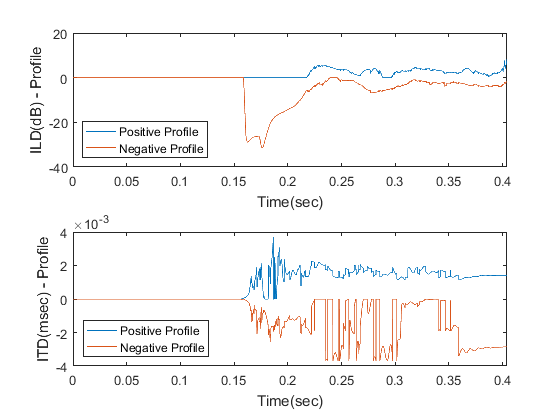
\includegraphics[width=\textwidth]{images/profiles_example.png}
  \caption{Προφίλ αμφιωτικών παραμέτρων: (Πάνω): ILD, (Κάτω): ITD.}
  \label{fig:profiles_example}
\end{figure}

\begin{CEquation}
\begin{split}
    CR = \frac{4*L}{N'_{dim}*L} = \frac{4}{N'_{dim}}
    \label{eq:compression_ratio}
\end{split}
\end{CEquation}